\documentclass[10pt]{article}
\usepackage[utf8]{inputenc}
\usepackage[includehead, headheight=10mm, margin=15mm ]{geometry}
\usepackage{amsmath}
\usepackage{amsthm}
\usepackage{amsfonts}
\usepackage{xcolor}
\usepackage{graphicx}
\usepackage{titling}
\usepackage{fancyhdr}
\usepackage{listings}
\usepackage{hyperref}
\usepackage{listings}


\title{APPM 4600 Lab 7}
\author{Edward Wawrzynek}
\date{10 October 2024}

\newcommand*{\dif}{\mathop{}\!\mathrm{d}}

\makeatletter
\def\@maketitle{%
  \newpage
  \null
  \vskip 1em%
  \begin{center}%
  \let \footnote \thanks
    {\LARGE \@title \par}%
    \vskip 1em%
    {\normalfont \@date}
  \end{center}%
  \par
  \vskip 1em}
\makeatother

\begin{document}

\pagestyle{fancy}
    \fancyhf{} % clear all header and footer fields
    \fancyhead[L]{\thetitle}
    \fancyhead[R]{\theauthor}

\makeatletter
\begin{center}
    {\Large \@title}
    \vskip 1mm
    {\normalfont \@date}
    \vskip 1em
\end{center}
\makeatother

The code for this lab can be seen on github \href{https://github.com/edwardwawrzynek/APPM4600/blob/master/Labs/Lab\%207/lab7.py}{here} and is included below.

\section{Prelab}
We have the polynomial \begin{align*}
    p_n(x) &= a_0 + a_1x + a_2x^2 + \dots + a_nx^n,
\end{align*} which we wish to use to interpolate the data \(\{x_j, f(x_j)\}_{j=0}^n\). We plug these data points into the polynomial and have the system \begin{align*}
    \vec{y} = V\vec{a},
\end{align*} where \(V\) is the vadermonde matrix \begin{align*}
    V = \begin{bmatrix}
      1 & x_1 & x_1^2 & \dots & x_1^n \\
      1 & x_2 & x_2^2 & \dots & x_2^n \\
      & & \dots \\
      1 & x_n & x_n^2 & \dots & x_n^n 
    \end{bmatrix}.
\end{align*} Thus, the coefficients \(\vec{a}\) are given by \begin{align*}
    \vec{a} = V^{-1}\vec{y}.
\end{align*}

\section{Different Interpolation Techniques}
The function \(f\) is interpolated with the three different methods. Results are shown below for different values of \(N\). Notice that the three methods generally give a very similar polynomial. This is expected, since we know that this polynomial is unique (this was shown in class).

\begin{center}
  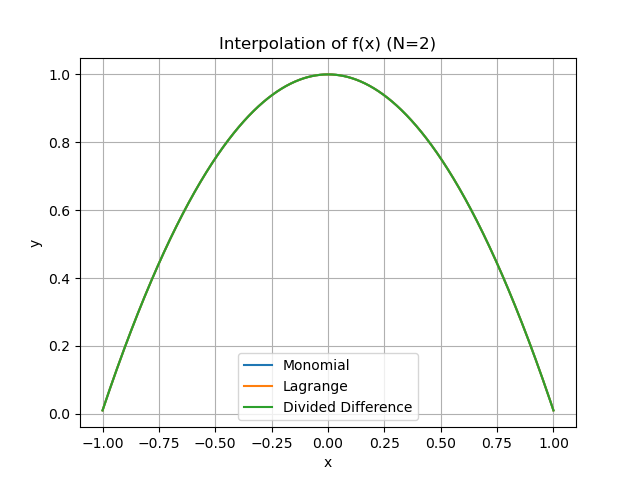
\includegraphics[width=0.45\textwidth]{lab7_interp_N2.png}
  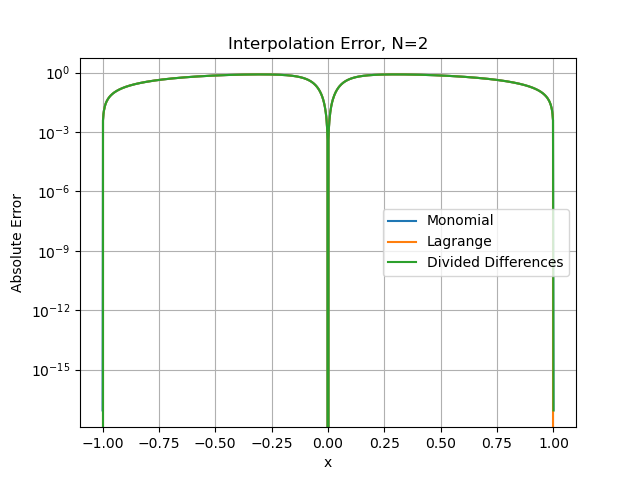
\includegraphics[width=0.45\textwidth]{lab7_interp_error_N2.png}

  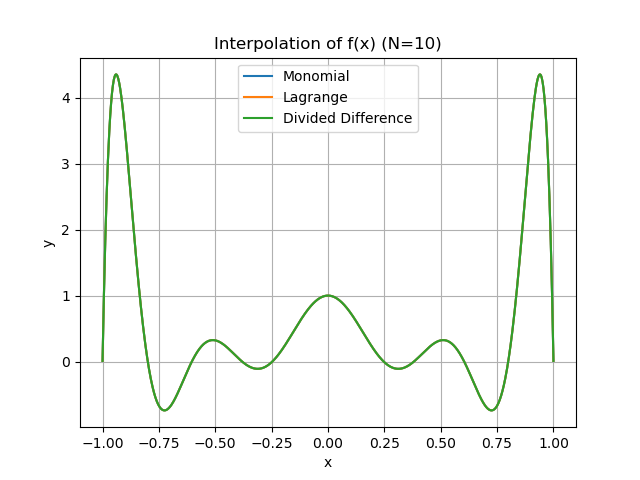
\includegraphics[width=0.45\textwidth]{lab7_interp_N10.png}
  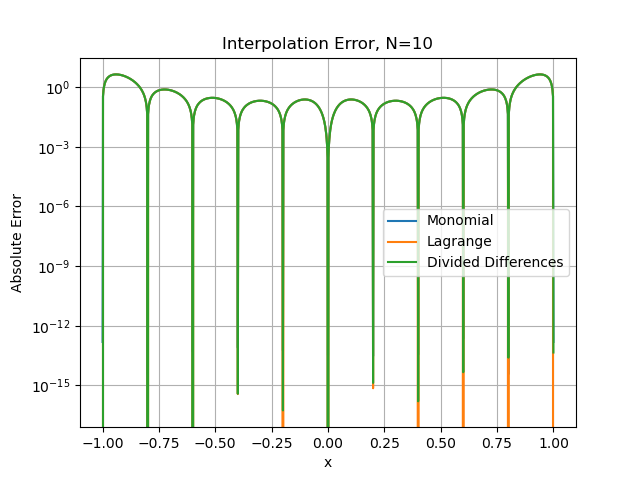
\includegraphics[width=0.45\textwidth]{lab7_interp_error_N10.png}
\end{center}

When \(N\) becomes large, the polynomials do a poor job of approximating the function near the edges of the domain. In particular, for \(N=19\) (shown below), the error grows very large near \(x=-1\) and \(x=1\). 

\begin{center}
  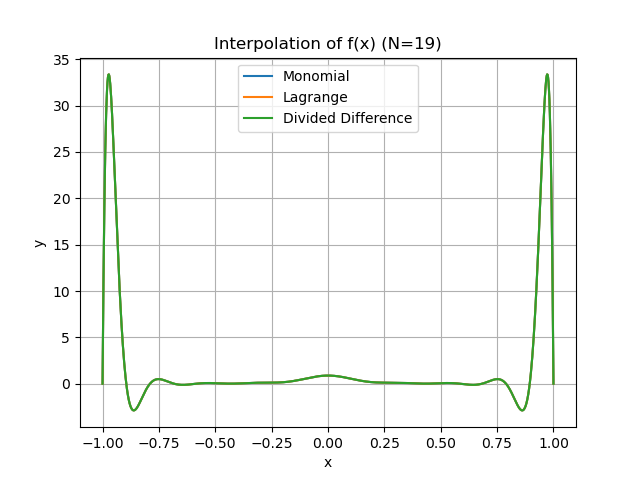
\includegraphics[width=0.45\textwidth]{lab7_interp_N19.png}
  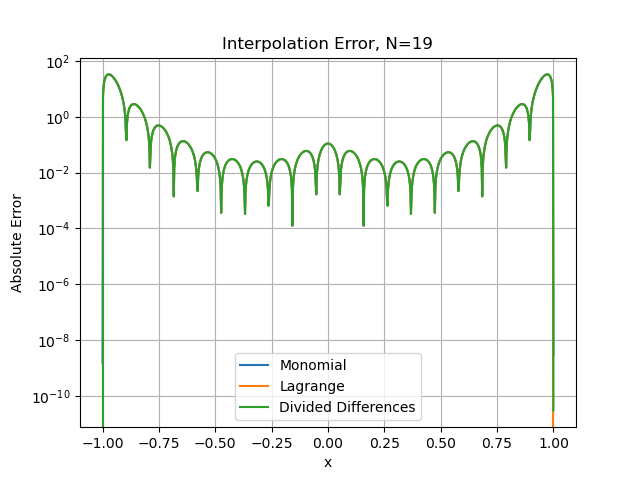
\includegraphics[width=0.45\textwidth]{lab7_interp_error_N19.png}
\end{center}

\section{Improving the approximation}
We place more points near the edges of the interval (as described in lab) and largely eliminate the \textit{Runge} phenomenon. Shown below is the result for \(N=19\) with more points at the edges of the domain. Notice that the error is smallest in the areas where we place more points.

\begin{center}
  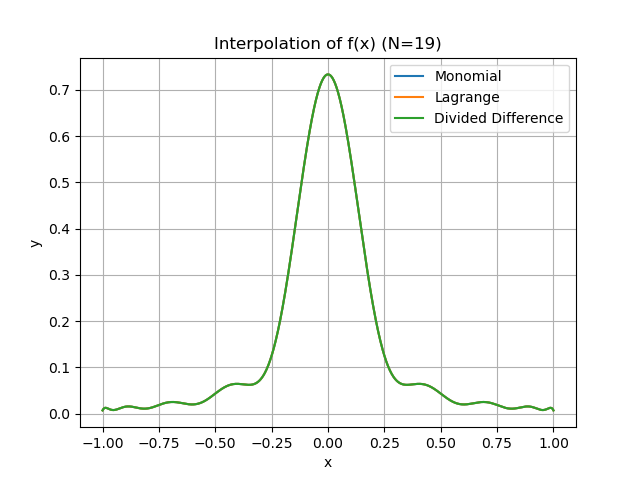
\includegraphics[width=0.45\textwidth]{lab7_uneven_interp_N19.png}
  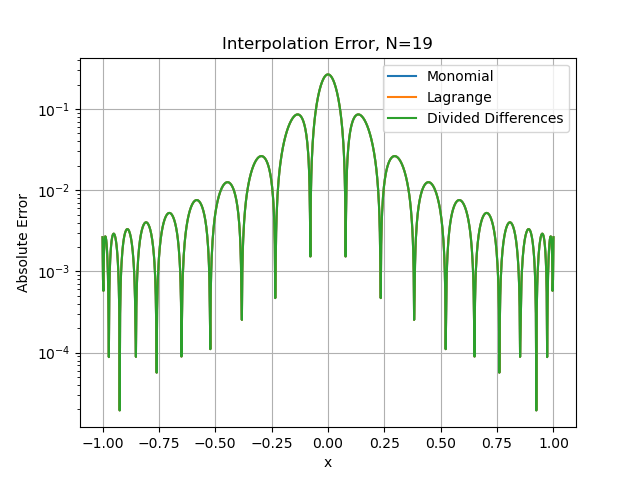
\includegraphics[width=0.45\textwidth]{lab7_uneven_interp_error_N19.png}
\end{center}

{\small \lstinputlisting[language=Python]{lab7.py}}   

\end{document}